\documentclass[preprint,3p,12pt,numbers]{elsarticle}
%% `numbers' selects natbib's numeric citation style internally.
%% Do not load natbib separately; elsarticle already loads it.

\usepackage{amsmath,amssymb,amsthm}
\usepackage{tikz}
\usepackage{booktabs}
\usepackage{hyperref}
\hypersetup{
  pdftitle={The Boolean Kernel Basis and Its Low-Degree Filtration over Arbitrary Fields},
  pdfauthor={Ali Mkhida (Algorizk Labs)},
  pdfsubject={Boolean kernel basis, polynomial degree filtration, and FRI-motivated algebra},
  pdfkeywords={finite fields, polynomial bases, Boolean lattice, Mobius transform, degree filtration, FRI},
  pdfdisplaydoctitle=true,
  bookmarks=true,
  bookmarksopen=true,
  bookmarksnumbered=true,
  linktoc=all,
  colorlinks=true,
  linkcolor=black,
  citecolor=black,
  urlcolor=blue
}
\urlstyle{same}

\newtheorem{theorem}{Theorem}[section]
\newtheorem{lemma}[theorem]{Lemma}
\newtheorem{proposition}[theorem]{Proposition}
\newtheorem{corollary}[theorem]{Corollary}
\theoremstyle{definition}
\newtheorem{definition}[theorem]{Definition}
\newtheorem{example}[theorem]{Example}
\theoremstyle{remark}
\newtheorem{remark}[theorem]{Remark}

\newcommand{\F}{\mathbb{F}}
\newcommand{\wt}{\mathrm{wt}}

\begin{document}

\begin{frontmatter}

\title{The Boolean Kernel Basis and Its Low-Degree Filtration over Arbitrary Fields}
\author[algorizk]{Ali Mkhida\corref{cor1}\fnref{orcid}}
\ead{ali.mkhida@algorizk.xyz}
\ead[url]{https://www.algorizk.xyz}
\cortext[cor1]{Corresponding author.}
\fntext[orcid]{ORCID: \href{https://orcid.org/0009-0009-2101-9070}{0009-0009-2101-9070}}
\fntext[website]{Extended research notes for this and related work:
\url{https://research.algorizk.xyz}.}

\address[algorizk]{Algorizk Labs\fnref{website}}

\begin{abstract}
For $N = 2^m$ and an arbitrary field $\mathbb{F}$, we study the family of
kernel polynomials $K_y(X) = \prod_{i=0}^{m-1}\left(X^{2^i}+y_i\right)$
indexed by $y \in \{0,1\}^m$. We show that this family is a basis of
$\mathbb{F}[X]_{<N}$ in which \emph{every} basis element has degree exactly
$N-1$: unlike degree-graded bases such as the monomial basis or the
Lin--Chung--Han novel polynomial basis, no element of the kernel basis has
low degree. We then characterize the ordinary degree filtration of
$\mathbb{F}[X]_{<N}$ directly in kernel coordinates. Writing each index as
$y = (x,h)$, with $x$ ranging over $k$ low coordinates and $h$ over the
remaining $q = m-k$ high coordinates, we prove that a polynomial $U$ has
degree less than $2^k$ if and only if its kernel-coefficient table
satisfies $\lambda_{(x,h)} = (-1)^{q-\wt(h)}\mu_x$ for a single function
$\mu$ on the low coordinates -- an alternating sign condition that is dual,
under the zeta/M\"obius transform on the Boolean lattice, to the trivial
vanishing of high monomial coefficients. We give both directions of this
equivalence, an explicit collapse formula recovering $U$ from $\mu$, and the
resulting subspace $CH_{m,k} \subset \mathbb{F}^{\{0,1\}^m}$ of dimension
$2^k$. All results hold over arbitrary fields, with no characteristic or
subspace assumption. A committed Rust implementation provides a reproducible computational cross-check of the coefficient transform and both directions of the filtration theorem, while a Lean~4 formalization is in progress and is not presented as a completed machine-checked proof.
\end{abstract}

\begin{keyword}
finite fields \sep polynomial bases \sep kernel polynomials \sep Boolean lattice \sep M\"obius transform \sep degree filtration
\end{keyword}

\end{frontmatter}

% Compact clickable navigation for the public ePrint/preprint version.
\begingroup
  \setcounter{tocdepth}{2}
  \small
  \tableofcontents
\endgroup
\medskip

\section{Introduction}
\label{sec:intro}

The relationship between a polynomial's degree and the coefficients that
describe it depends entirely on which basis those coefficients are taken
in. In the monomial basis $\{1,X,X^2,\dots\}$ this relationship is
definitional: $U$ has degree less than $2^k$ exactly when its coefficients
on monomials of degree $2^k$ and above vanish. Every \emph{degree-graded}
basis of $\mathbb{F}[X]_{<N}$ -- one in which the $j$-th basis element has
degree $j$ -- inherits the same picture for free: sparsity of the
coefficient table above index $2^k-1$ is the degree bound.

This paper studies a basis for which that picture fails completely. Index
$\mathbb{F}[X]_{<N}$, $N=2^m$, by Boolean vectors $y \in \{0,1\}^m$ via the
kernel polynomials
\[
  K_y(X) = \prod_{i=0}^{m-1} \left(X^{2^i}+y_i\right) .
\]
Theorem~\ref{thm:basis} shows $\{K_y\}$ is a basis of $\mathbb{F}[X]_{<N}$
over an arbitrary field $\mathbb{F}$, with no assumption on characteristic.
But every single kernel polynomial has degree exactly $N-1$
(Proposition~\ref{prop:kernel-degree}): the basis is maximally degenerate
with respect to degree, and no sub-collection of its elements spans a
proper degree-filtered subspace. If a polynomial $U$ has small degree,
that fact cannot show up as \emph{which} kernel coefficients are zero,
because none of the individual basis elements are themselves low-degree.

Our main result, Theorem~\ref{thm:filtration}, identifies what a degree
bound looks like instead. Splitting a kernel index $y=(x,h)$ into $k$ low
coordinates and $q=m-k$ high coordinates, $U$ has degree less than $2^k$
if and only if its kernel coefficients satisfy
\[
  \lambda_{(x,h)} = (-1)^{q-\wt(h)}\, \mu_x
\]
for a single function $\mu$ of the low coordinates alone -- an alternating
sign condition across every fiber of the high coordinates, rather than a
support condition. This is the Boolean-lattice M\"obius dual of the
trivial monomial statement: where the monomial basis reads off degree as
which coefficients vanish, the kernel basis reads off degree as a rigid
sign pattern relating the coefficients that remain.

Bases indexed by $\{0,1\}^m$ and built from a per-coordinate recursive
product are not new in themselves: the Lin--Chung--Han ``novel polynomial
basis'' \citep{LinChungHan2014} plays a comparable role in additive Fourier
transforms over characteristic-two fields, and underlies the folding step
of recent FRI-based polynomial commitment schemes
\citep{ZeilbergerChenFisch2024Basefold,DiamondPosen2026FRIBinius}.
Section~\ref{sec:related} makes the comparison precise; in short, the
Lin--Chung--Han basis is degree-graded and tied to a chosen subspace
structure over a field of characteristic two, so its interaction with
degree is the ordinary sparsity picture. The kernel basis studied here is
field-agnostic and maximally degenerate in degree instead, which is
exactly what makes Theorem~\ref{thm:filtration} necessary rather than
immediate. We view the degree-halving behavior of an FRI-style folding
step as a natural setting where a result like
Theorem~\ref{thm:filtration} may be put to use. This paper is
self-contained and establishes the underlying algebra on its own terms.

\paragraph{Contributions}
\begin{itemize}
\item We prove that the kernel polynomials $\{K_y : y \in \{0,1\}^m\}$
  form a basis of $\mathbb{F}[X]_{<N}$ over an arbitrary field, and that
  every element of this basis has degree exactly $N-1$
  (Theorem~\ref{thm:basis}, Proposition~\ref{prop:kernel-degree}).
\item We give the exact change of basis relating kernel and monomial
  coordinates, as a Boolean zeta transform composed with a complement
  permutation, invertible by Boolean M\"obius inversion in
  $O(N \log N)$ operations (Section~\ref{subsec:zeta}).
\item We characterize the ordinary degree filtration of
  $\mathbb{F}[X]_{<N}$ exactly in kernel coordinates, as an
  alternating-sign condition rather than a sparsity condition
  (Theorem~\ref{thm:filtration}), together with an explicit collapse
  formula (Proposition~\ref{prop:collapse}) and the resulting
  $2^k$-dimensional subspace $CH_{m,k}$ (Corollary~\ref{cor:CH}).
\item We provide a committed Rust cross-check of the coefficient
  formula, zeta/M\"obius transforms, and both directions of the filtration
  theorem over the Goldilocks prime field, and report separately on an
  in-progress Lean~4 formalization whose proofs are not yet complete
  (Section~\ref{sec:verification}).
\end{itemize}

\paragraph{Organization}
Section~\ref{sec:related} positions this work against the closest prior
constructions. Section~\ref{sec:prelim} fixes notation and records the
(standard) monomial picture of the degree filtration.
Section~\ref{sec:basis} defines the kernel basis and proves
Theorem~\ref{thm:basis}. Section~\ref{sec:filtration} is the paper's core,
proving Theorem~\ref{thm:filtration}. Section~\ref{sec:verification}
records the state of computational and formal verification, and
Section~\ref{sec:conclusion} closes with directions for future work.

\section{Related work}
\label{sec:related}

\paragraph{The Lin--Chung--Han novel polynomial basis}
A relevant comparison is the ``novel polynomial basis''
of Lin, Chung, and Han \citep{LinChungHan2014}, developed for additive
Fourier transforms over characteristic-two fields. Fixing a Cantor basis
of $\mathbb{F}_{2^r}$ and the associated subspace-vanishing polynomials
$s_0, s_1, \dots$, their basis elements are $X_j(x) = \prod_i s_i(x)^{b_i}$
for $j = \sum_i b_i 2^i$, and satisfy $\deg X_j = j$: the basis is
degree-graded, so low degree is exactly sparsity, the same relationship
the monomial basis already gives for free. The kernel basis differs on
every axis that matters here: it requires no characteristic assumption
and no chosen subspace of a field extension, being built instead from
literal power-of-$X$ shifts; and every element has degree $N-1$ regardless
of index, so no element is itself low-degree. Theorem~\ref{thm:filtration}
exists because the kernel basis is degree-degenerate in a way the
Lin--Chung--Han basis is not.

% CHAR2_BERNSTEIN_RELATION_2026_08_16
\paragraph{Scaled Bernstein specialization in characteristic two}
There is an exact classical specialization when
$\operatorname{char}\mathbb{F}=2$. Set $n=N-1=2^m-1$ and
$j=|y|_2$. Since $X^{2^i}+1=(X+1)^{2^i}$ in characteristic two,
\[
  K_y(X)=X^{\,n-j}(X+1)^j=X^{\,n-j}(1-X)^j .
\]
Thus, after the reindexing $i=n-j$, the kernel family is exactly the
scaled Bernstein basis
$\varphi_{i,n}(X;0,1)=X^i(1-X)^{n-i}$ of grade $n$; see, for example,
Mackey and Perovi\'c \citep{MackeyPerovic2016}. In this particular grade
the usual Bernstein binomial normalization also disappears modulo two:
in $\mathbb{F}_2[T]$,
\[
  (1+T)^{2^m-1}=1+T+\cdots+T^{2^m-1},
\]
so every coefficient $\binom{2^m-1}{j}$ is $1$ modulo $2$. This
identifies a classical boundary case of the construction. The
arbitrary-field filtration theorem below does not rely on characteristic
two.

\paragraph{The Boolean zeta and M\"obius transforms}
The change of basis underlying Section~\ref{sec:basis} -- summing kernel
coefficients over a superset in the Boolean lattice, and inverting by an
alternating sum -- is the classical zeta transform and its M\"obius
inversion on the subset lattice, foundational to enumerative combinatorics
and, under the name of the algebraic-normal-form transform, to the
analysis of Boolean functions over $\mathbb{F}_2$. What is not classical,
to the best of our knowledge, is the specific fact that this transform,
composed with a fixed complement permutation and specialized to the
maximally-degenerate kernel basis, characterizes the ordinary polynomial
degree filtration via an alternating sign condition rather than a support
condition. We were unable to locate this statement, or an evidently
equivalent one, in the additive-FFT or coding-theory literature;
Section~\ref{sec:filtration} states and proves it directly.

\paragraph{FRI and folding-based polynomial commitments}
Fast Reed--Solomon Interactive Oracle Proofs of Proximity (FRI)
\citep{BenSassonEtAl2018FRI} test proximity to a low-degree Reed--Solomon
codeword by repeatedly folding a polynomial via its even and odd parts,
halving the degree bound at each round. BaseFold
\citep{ZeilbergerChenFisch2024Basefold} generalizes this folding step to
arbitrary fields via foldable codes, and FRI-Binius
\citep{DiamondPosen2026FRIBinius} draws an explicit connection between an
additive transform built on the Lin--Chung--Han basis and binary-field
FRI, prescribing concrete choices left generic in the original
construction. Both lines of work establish degree-halving under folding
directly, without passing through an intermediate basis-theoretic
statement of the kind given here. This paper does not attempt a new folding or proximity result; the interaction of the even--odd folding operator with the kernel coefficient table is left to future work.

\section{Preliminaries}
\label{sec:prelim}

Throughout, $\mathbb{F}$ denotes an arbitrary field: no assumption is made
on its characteristic. Fix an integer $m \geq 1$ and set
\[
  N = 2^m, \qquad \mathbb{B}^m = \{0,1\}^m .
\]
We write $\mathbb{F}[X]_{<N}$ for the $N$-dimensional $\mathbb{F}$-vector
space of polynomials of degree strictly less than $N$.

\subsection{Binary exponent coordinates}
\label{subsec:binary}

For $a = (a_0,\dots,a_{m-1}) \in \mathbb{B}^m$, define its binary value
\[
  |a|_2 = \sum_{i=0}^{m-1} a_i 2^i .
\]
The map $a \mapsto |a|_2$ is a bijection $\mathbb{B}^m \to \{0,\dots,N-1\}$,
so every polynomial $U \in \mathbb{F}[X]_{<N}$ has a unique expansion
\[
  U(X) = \sum_{a \in \mathbb{B}^m} u_a X^{|a|_2},
\]
a reindexing of the ordinary monomial coefficients by Boolean vectors rather
than by integers, not a new representation of $U$.

For $a, y \in \mathbb{B}^m$ we write $y \geq a$ when $y_i \geq a_i$ for
every coordinate $i$, and we let $\wt(y) = \sum_i y_i$ denote the Hamming
weight of $y$.

Fix $0 \leq k \leq m$ and set $q = m-k$. Every $a \in \mathbb{B}^m$
decomposes uniquely as $a = (r,s)$ with $r \in \mathbb{B}^k$ the low
coordinates and $s \in \mathbb{B}^{q}$ the high coordinates, and
\[
  |a|_2 = |r|_2 + 2^k |s|_2 .
\]

\begin{proposition}[Monomial low-degree condition]
\label{prop:monomial-degree}
Write
\[
  U(X) =
  \sum_{(r,s) \in \mathbb{B}^k \times \mathbb{B}^{q}}
  u_{(r,s)}\, X^{|r|_2 + 2^k|s|_2}.
\]
Then $\deg U < 2^k$ if and only if
$u_{(r,s)} = 0$ for every $r \in \mathbb{B}^k$ and every nonzero
$s \in \mathbb{B}^{q}$.
\end{proposition}

\begin{proof}
If $\deg U < 2^k$ and $s \neq 0$, then $|s|_2 \geq 1$, so
$|r|_2 + 2^k|s|_2 \geq 2^k$ for every $r$, and the corresponding monomial
cannot occur in $U$; hence $u_{(r,s)}=0$. Conversely, if $u_{(r,s)}=0$
whenever $s \neq 0$, then
$U(X) = \sum_{r \in \mathbb{B}^k} u_{(r,0)} X^{|r|_2}$ with
$|r|_2 \leq 2^k-1$ for every $r$, so $\deg U < 2^k$.
\end{proof}

Proposition~\ref{prop:monomial-degree} is the ordinary, sparsity-based
picture of the degree filtration on $\mathbb{F}[X]_{<N}$: a degree bound
is equivalent to the vanishing of a set of monomial coefficients. Every
degree-graded basis of $\mathbb{F}[X]_{<N}$ shares this picture. Section~
\ref{sec:basis} introduces a basis for which it fails completely, and
Section~\ref{sec:filtration} identifies what replaces it.

\section{The Boolean kernel basis}
\label{sec:basis}

\subsection{Definition and degree}
\label{subsec:def-degree}

\begin{definition}[Kernel polynomial]
\label{def:kernel}
For $y = (y_0,\dots,y_{m-1}) \in \mathbb{B}^m$, the associated
\emph{kernel polynomial} is
\[
  K_y(X) = \prod_{i=0}^{m-1} \left( X^{2^i} + y_i \right) \in \mathbb{F}[X].
\]
\end{definition}

Every factor $X^{2^i}+y_i$ is monic of degree $2^i$.

\begin{proposition}[Every kernel polynomial has maximal degree]
\label{prop:kernel-degree}
For every $y \in \mathbb{B}^m$, $\deg K_y = N-1$, with leading coefficient
$1$.
\end{proposition}

\begin{proof}
Selecting the term $X^{2^i}$ from every factor gives the monomial
$\prod_{i=0}^{m-1} X^{2^i} = X^{\sum_i 2^i} = X^{N-1}$ with coefficient
$1$; any other choice of terms from the factors yields a monomial of
strictly lower degree, so it cannot cancel the leading term.
\end{proof}

Proposition~\ref{prop:kernel-degree} is what distinguishes the kernel basis
from degree-graded bases of $\mathbb{F}[X]_{<N}$, including the monomial
basis and the Lin--Chung--Han novel polynomial basis discussed in
Section~\ref{sec:related}: \emph{every} kernel polynomial sits at the top
of the degree range, so no element of the basis is itself low-degree. A
degree bound on $U$ can therefore not be read off as sparsity of its kernel
coefficients, the way it can for a degree-graded basis
(Proposition~\ref{prop:monomial-degree}). Section~\ref{sec:filtration}
identifies exactly what a degree bound looks like in this basis instead.

\subsection{Exact coefficient formula}
\label{subsec:coeff-formula}

For $a \in \mathbb{B}^m$, write $K_y(X) = \sum_{a \in \mathbb{B}^m}
[K_y]_a \, X^{|a|_2}$.

\begin{proposition}[Coefficient formula]
\label{prop:coeff-formula}
For every $a, y \in \mathbb{B}^m$, write $\bar a = (1-a_0,\dots,1-a_{m-1})$
for the Boolean complement of $a$. Then
\[
  [K_y]_a = \prod_{i \,:\, a_i = 0} y_i =
  \begin{cases} 1, & y \geq \bar a, \\ 0, & \text{otherwise.} \end{cases}
\]
\end{proposition}

\begin{proof}
The monomial $X^{|a|_2}$ arises from the product by choosing $X^{2^i}$
from the $i$-th factor whenever $a_i=1$, and choosing the constant term
$y_i$ whenever $a_i=0$; the resulting coefficient is
$\prod_{i \,:\, a_i=0} y_i$. Since each $y_i \in \{0,1\}$, this product
equals $1$ exactly when $y_i=1$ for every $i$ with $a_i=0$. As
$\bar a_i = 1$ exactly when $a_i=0$ (and imposes no constraint when
$\bar a_i=0$), this condition is exactly $y_i \geq \bar a_i$ for every
$i$, i.e.\ $y \geq \bar a$.
\end{proof}

Consequently $\mathrm{Supp}(K_y) = \{a \in \mathbb{B}^m : y \geq \bar a\}$
has size $2^{\wt(y)}$: the condition $y \geq \bar a$ says
$y_i + a_i \geq 1$ for every $i$, so each coordinate with $y_i=0$ forces
$a_i=1$ on the support, while each coordinate with $y_i=1$ leaves $a_i$
free.

\begin{example}
\label{ex:m2}
For $m=2$ ($N=4$): $K_{(0,0)}(X) = X^3$, $K_{(1,0)}(X) = X^3+X^2$,
$K_{(0,1)}(X) = X^3+X$, and $K_{(1,1)}(X) = X^3+X^2+X+1$. The two extremal
indices give $K_{0^m}(X) = X^{N-1}$ and
$K_{1^m}(X) = 1+X+\cdots+X^{N-1}$, related by
$(X-1)K_{1^m}(X) = X^N-1$.
\end{example}

\subsection{Recursive decomposition and the basis theorem}
\label{subsec:basis-thm}

Write $y = (b,z)$ with $b = y_0 \in \{0,1\}$ and
$z = (y_1,\dots,y_{m-1}) \in \mathbb{B}^{m-1}$, and let
$K_z(Y) = \prod_{i=0}^{m-2} (Y^{2^i}+z_i)$ be the corresponding kernel
polynomial for $m-1$. Substituting $Y=X^2$ gives
\begin{equation}
\label{eq:recursion}
  K_{(0,z)}(X) = X\, K_z(X^2), \qquad
  K_{(1,z)}(X) = (X+1)\, K_z(X^2),
\end{equation}
splitting every kernel polynomial into an even part and an odd part in $X$.

\begin{theorem}[Boolean kernel basis]
\label{thm:basis}
The family $\{K_y(X) : y \in \mathbb{B}^m\}$ is a basis of
$\mathbb{F}[X]_{<N}$.
\end{theorem}

\begin{proof}
Both sides have dimension $N=2^m$, so it suffices to prove linear
independence, by induction on $m$. For $m=1$, $K_{(0)}(X)=X$ and
$K_{(1)}(X)=X+1$ are linearly independent. Assume the claim for $m-1$ and
suppose
\[
  \sum_{z \in \mathbb{B}^{m-1}} \alpha_{0,z}\, K_{(0,z)}(X)
  + \sum_{z \in \mathbb{B}^{m-1}} \alpha_{1,z}\, K_{(1,z)}(X) = 0 .
\]
By~\eqref{eq:recursion} this reads
\[
  \sum_z \alpha_{1,z}\, K_z(X^2)
  \;+\; X \sum_z (\alpha_{0,z}+\alpha_{1,z})\, K_z(X^2) = 0 .
\]
The first sum contains only even powers of $X$ and the second only odd
powers, so each must vanish separately. By the induction hypothesis the
polynomials $K_z(Y)$, $z \in \mathbb{B}^{m-1}$, are linearly independent in
$Y$, so evaluating at $Y=X^2$ preserves their independence and forces
$\alpha_{1,z}=0$ for every $z$; the second identity then gives
$\alpha_{0,z}=0$ as well.
\end{proof}

Every $U \in \mathbb{F}[X]_{<N}$ therefore has a unique kernel expansion
$U(X) = \sum_{y \in \mathbb{B}^m} \lambda_y K_y(X)$; we call
$\lambda : \mathbb{B}^m \to \mathbb{F}$ the \emph{kernel coefficient table}
of $U$. These are coordinates of $U$ in the basis $\{K_y\}$, and should not
be confused with values of $U$ at points of $\mathbb{F}$.

\subsection{The zeta transform between kernel and monomial coordinates}
\label{subsec:zeta}

Comparing the two expansions of $U$ via Proposition~\ref{prop:coeff-formula}
gives
\begin{equation}
\label{eq:zeta}
  u_a = \sum_{y \geq \bar a} \lambda_y ,
\end{equation}
the Boolean zeta transform of $\lambda$, evaluated at the complement of
$a$. Writing $\zeta\lambda(c) := \sum_{y \geq c} \lambda_y$ for the
ordinary zeta transform of $\lambda$ on the Boolean lattice,
\eqref{eq:zeta} says $u_a = \zeta\lambda(\bar a)$: the monomial
coefficients are the zeta transform of $\lambda$, followed by the
complement permutation $a \mapsto \bar a$.

In matrix form $u = Z_m \lambda$ with
$Z_m(a,y) = \mathbf{1}[y \geq \bar a]$; for $m=1$,
$Z_1 = \left(\begin{smallmatrix} 0 & 1 \\ 1 & 1 \end{smallmatrix}\right)$
has $\det Z_1 = -1$, and $Z_m$ is, up to the ordering of Boolean indices,
the $m$-fold Kronecker power of $Z_1$ -- hence invertible over every field.
This furnishes a second, purely linear-algebraic proof of
Theorem~\ref{thm:basis}.

Ordinary Boolean M\"obius inversion recovers $\lambda$ from $\zeta\lambda$,
$\lambda_y = \sum_{b \geq y} (-1)^{\wt(b)-\wt(y)} \zeta\lambda(b)$;
substituting $\zeta\lambda(b) = u_{\bar b}$ from~\eqref{eq:zeta} gives
\begin{equation}
\label{eq:mobius}
  \lambda_y = \sum_{b \geq y} (-1)^{\wt(b)-\wt(y)}\, u_{\bar b} ,
\end{equation}
an identity that remains valid in characteristic $2$, where addition and
subtraction coincide. Both the zeta transform and M\"obius inversion
evaluate coordinate by coordinate on the standard butterfly schedule for
the Boolean lattice, in $\tfrac{1}{2} N \log_2 N$ field operations each --
that is, $O(N \log N)$ total for~\eqref{eq:zeta} or~\eqref{eq:mobius}
together with the free $O(N)$ relabeling $a \mapsto \bar a$, rather than
the $O(N^2)$ of a naive change of basis -- confirmed empirically in
Section~\ref{sec:verification}.

\section{The low-degree filtration}
\label{sec:filtration}

This section states and proves the paper's main result: an exact
characterization of the degree filtration of $\mathbb{F}[X]_{<N}$ directly
in kernel coordinates. By Proposition~\ref{prop:kernel-degree}, no single
kernel polynomial is low-degree, so this cannot be a sparsity condition on
$\lambda$ the way Proposition~\ref{prop:monomial-degree} is a sparsity
condition on $u$; Theorem~\ref{thm:filtration} identifies the condition
that replaces it.

\subsection{Setting and the high-coordinate sign character}
\label{subsec:filt-setting}

Fix $0 \leq k \leq m$ and set $q=m-k$, exactly as in
Section~\ref{sec:prelim}, but now split the \emph{kernel} index
$y \in \mathbb{B}^m$ rather than the monomial index: write $y=(x,h)$ with
$x \in \mathbb{B}^k$ the low coordinates and $h \in \mathbb{B}^{q}$ the
high coordinates, and write the kernel expansion of $U$ accordingly,
\[
  U(X) = \sum_{(x,h) \in \mathbb{B}^k \times \mathbb{B}^{q}}
  \lambda_{(x,h)}\, K_{(x,h)}(X) .
\]

\begin{definition}[High-coordinate sign character]
\label{def:character}
For $h \in \mathbb{B}^{q}$, set $\sigma_q(h) = (-1)^{q-\wt(h)}$.
Equivalently $\sigma_q(h) = \prod_{j=0}^{q-1}(-1)^{1-h_j}$: the sign flips
whenever a single high coordinate is flipped. Up to the constant factor
$(-1)^q$, $\sigma_q$ is the Boolean character $h \mapsto (-1)^{\wt(h)}$.
\end{definition}

\subsection{The main theorem}
\label{subsec:main-thm}

\begin{theorem}[Low-degree filtration]
\label{thm:filtration}
Let $U(X) = \sum_{(x,h)} \lambda_{(x,h)} K_{(x,h)}(X) \in \mathbb{F}[X]_{<N}$.
Then $\deg U < 2^k$ if and only if there is a (necessarily unique) function
$\mu : \mathbb{B}^k \to \mathbb{F}$ with
\[
  \lambda_{(x,h)} = (-1)^{q-\wt(h)}\, \mu_x
  \qquad \text{for every } x \in \mathbb{B}^k,\ h \in \mathbb{B}^{q} .
\]
When it exists, $\mu_x = \lambda_{(x,1_{q})}$, where $1_{q}$ denotes the
all-ones vector of $\mathbb{B}^{q}$.
\end{theorem}

\subsection{Proof: degree implies the character condition}
\label{subsec:proof-forward}

Write the monomial expansion of $U$ along the same low/high split,
as in Proposition~\ref{prop:monomial-degree}:
\[
  U(X) =
  \sum_{(r,s)} u_{(r,s)}\, X^{|r|_2+2^k|s|_2}.
\] Splitting the zeta
transform~\eqref{eq:zeta} along these blocks, with $\bar r \in \mathbb{B}^k$
and $\bar s \in \mathbb{B}^{q}$ the complements of $r$ and $s$,
\begin{equation}
\label{eq:block-zeta}
  u_{(r,s)} = \sum_{x \geq \bar r}\ \sum_{h \geq \bar s} \lambda_{(x,h)} .
\end{equation}

\begin{proof}[Proof of Theorem~\ref{thm:filtration}, forward direction]
Suppose $\deg U < 2^k$. By Proposition~\ref{prop:monomial-degree},
$u_{(r,s)}=0$ for every $r \in \mathbb{B}^k$ and every nonzero
$s \in \mathbb{B}^{q}$. Fix such an $s$ and, for $x \in \mathbb{B}^k$, set
$F(x) = \sum_{h \geq \bar s} \lambda_{(x,h)}$, so by~\eqref{eq:block-zeta},
$u_{(r,s)} = \sum_{x \geq \bar r} F(x)$ for every $r$. As $r$ ranges over
$\mathbb{B}^k$ so does $\bar r$, so $u_{(r,s)}=0$ for every $r$ says that
the zeta transform of $F$ on $\mathbb{B}^k$ vanishes identically; since
that transform is invertible (Section~\ref{subsec:zeta}), $F \equiv 0$.
Thus
\begin{equation}
\label{eq:Gx-vanish}
  \sum_{h \geq \bar s} \lambda_{(x,h)} = 0
  \qquad \text{for every } x \in \mathbb{B}^k
  \text{ and every nonzero } s \in \mathbb{B}^{q} .
\end{equation}
Fix $x$ and define $G_x(b) = \sum_{h \geq b} \lambda_{(x,h)}$ for
$b \in \mathbb{B}^{q}$. As $s$ ranges over the nonzero vectors of
$\mathbb{B}^{q}$, its complement $\bar s$ ranges over every vector of
$\mathbb{B}^{q}$ except $1_{q}$, so \eqref{eq:Gx-vanish} says exactly
$G_x(b)=0$ for every $b \neq 1_{q}$. Boolean M\"obius inversion recovers
$\lambda_{(x,h)}$ from $G_x$,
$\lambda_{(x,h)} = \sum_{b \geq h}(-1)^{\wt(b)-\wt(h)} G_x(b)$; since $G_x$
vanishes except at $b=1_{q}$, only that term survives:
\[
  \lambda_{(x,h)} = (-1)^{\wt(1_{q})-\wt(h)}\, G_x(1_{q})
  = (-1)^{q-\wt(h)}\, \mu_x , \qquad
  \mu_x := G_x(1_{q}) = \lambda_{(x,1_{q})} .
\]
\end{proof}

\subsection{Proof: the character condition implies low degree}
\label{subsec:proof-converse}

\begin{proof}[Proof of Theorem~\ref{thm:filtration}, converse direction]
Suppose $\lambda_{(x,h)} = (-1)^{q-\wt(h)}\mu_x$ for every $x,h$. Let
$s \in \mathbb{B}^{q}$ be nonzero and set $b=\bar s$; since $s \neq 0_{q}$,
$b \neq 1_{q}$, so $b$ has at least one zero coordinate -- say
$f \geq 1$ of them. For every $x$,
\[
  \sum_{h \geq b} \lambda_{(x,h)} = \mu_x \sum_{h \geq b} (-1)^{q-\wt(h)} .
\]
Writing $h=b$ plus an arbitrary assignment of the $f$ free coordinates,
$\sum_{h \geq b}(-1)^{q-\wt(h)} = (-1)^{q-\wt(b)}\sum_{j=0}^{f}\binom{f}{j}
(-1)^{j} = (-1)^{q-\wt(b)}(1-1)^{f} = 0$ since $f \geq 1$. Hence
$\sum_{h \geq \bar s}\lambda_{(x,h)}=0$ for every $x$ and every nonzero
$s$, and by~\eqref{eq:block-zeta}, $u_{(r,s)}=0$ for every $r$ and every
nonzero $s$. Proposition~\ref{prop:monomial-degree} then gives
$\deg U < 2^k$.
\end{proof}

Uniqueness of $\mu$ in Theorem~\ref{thm:filtration} is immediate from the
forward direction: $\mu_x$ is forced to equal $\lambda_{(x,1_q)}$.

\subsection{Collapse of the high coordinates}
\label{subsec:collapse}

For $x \in \mathbb{B}^k$, define the truncated kernel polynomial
\[
  K_x^{[k]}(X) = \prod_{i=0}^{k-1} \left( X^{2^i}+x_i \right) ,
\]
the degree-$(2^k-1)$ kernel polynomial for $m=k$ built from only the low
coordinates.

\begin{proposition}[Collapse formula]
\label{prop:collapse}
If $\deg U < 2^k$, then
$U(X) = \sum_{x \in \mathbb{B}^k} \mu_x\, K_x^{[k]}(X)$, with $\mu$ as in
Theorem~\ref{thm:filtration}.
\end{proposition}

\begin{proof}
By Theorem~\ref{thm:filtration},
$U(X) = \sum_{x} \mu_x \sum_{h \in \mathbb{B}^{q}} (-1)^{q-\wt(h)}
K_{(x,h)}(X)$. Since
$K_{(x,h)}(X) = K_x^{[k]}(X) \cdot \prod_{j=0}^{q-1}
\left(X^{2^{k+j}}+h_j\right)$, and $(-1)^{q-\wt(h)} =
\prod_{j=0}^{q-1}(-1)^{1-h_j}$ by Definition~\ref{def:character}, the
inner sum factors coordinate by coordinate:
\[
  \sum_{h \in \mathbb{B}^{q}} (-1)^{q-\wt(h)} K_{(x,h)}(X)
  = K_x^{[k]}(X) \prod_{j=0}^{q-1}
  \left[ \sum_{h_j \in \{0,1\}} (-1)^{1-h_j}
  \left(X^{2^{k+j}}+h_j\right) \right] .
\]
Each bracketed factor equals
$-\!\left(X^{2^{k+j}}+0\right) + \left(X^{2^{k+j}}+1\right) = 1$, so the
product is $K_x^{[k]}(X)$ and $U(X) = \sum_x \mu_x K_x^{[k]}(X)$.
\end{proof}

\subsection{The character-side low-degree space}
\label{subsec:CH}

\begin{definition}
\label{def:CH}
\[
  CH_{m,k} = \left\{ \lambda \in \mathbb{F}^{\mathbb{B}^m} :
  \lambda_{(x,h)} = (-1)^{q-\wt(h)}\mu_x \text{ for some }
  \mu : \mathbb{B}^k \to \mathbb{F} \right\} .
\]
\end{definition}

\begin{corollary}
\label{cor:CH}
$\deg U < 2^k \iff \lambda \in CH_{m,k}$, and $\dim CH_{m,k} = 2^k$.
\end{corollary}

\begin{proof}
The equivalence is Theorem~\ref{thm:filtration}. The map
$\mu \mapsto \lambda$ of Definition~\ref{def:CH} is linear and, by the
uniqueness clause of Theorem~\ref{thm:filtration}, injective, with image
exactly $CH_{m,k}$; hence $\dim CH_{m,k} = \dim \mathbb{F}^{\mathbb{B}^k}
= 2^k$, matching $\dim \mathbb{F}[X]_{<2^k}=2^k$.
\end{proof}

\subsection{Worked example: $m=3$, $k=1$}
\label{subsec:example-filt}

Here $q=2$. Table~\ref{tab:example} lists the character value
$\sigma_2(h)=(-1)^{2-\wt(h)}$ for each $h \in \mathbb{B}^2$ and the
resulting kernel coefficient in the fiber over a fixed $x$.

\begin{table}[h]
\centering
\begin{tabular}{ccc}
\toprule
$h$ & $\sigma_2(h)$ & $\lambda_{(x,h)}$ \\
\midrule
$(0,0)$ & $1$  & $\mu_x$  \\
$(1,0)$ & $-1$ & $-\mu_x$ \\
$(0,1)$ & $-1$ & $-\mu_x$ \\
$(1,1)$ & $1$  & $\mu_x$  \\
\bottomrule
\end{tabular}
\caption{The character condition for $q=2$.}
\label{tab:example}
\end{table}

Figure~\ref{fig:cube} shows the same data laid out on the Boolean square
$\mathbb{B}^2$: an edge flips one coordinate of $h$, and the sign flips
with it, so the character condition colors $\mathbb{B}^2$ like a
checkerboard, $\mu_x$ on one part and $-\mu_x$ on the other. The same
holds on $\mathbb{B}^q$ for any $q$: adjacent vertices (differing in one
coordinate) always carry opposite signs, since flipping a single
coordinate of $h$ changes $\wt(h)$ by exactly $1$.

\begin{figure}[h]
\centering
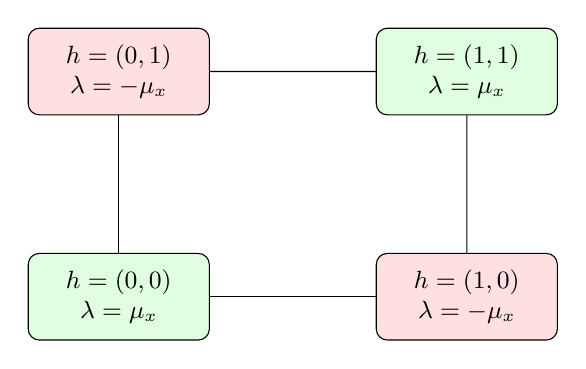
\begin{tikzpicture}[scale=1.3,
  vert/.style={draw, rectangle, rounded corners, minimum width=2.3cm,
    minimum height=1.1cm, align=center, font=\small}]
  \node[vert, fill=green!12] (00) at (0,0)    {$h=(0,0)$\\ $\lambda=\mu_x$};
  \node[vert, fill=red!12]   (10) at (3.4,0)  {$h=(1,0)$\\ $\lambda=-\mu_x$};
  \node[vert, fill=red!12]   (01) at (0,2.2)  {$h=(0,1)$\\ $\lambda=-\mu_x$};
  \node[vert, fill=green!12] (11) at (3.4,2.2){$h=(1,1)$\\ $\lambda=\mu_x$};
  \draw (00) -- (10);
  \draw (00) -- (01);
  \draw (10) -- (11);
  \draw (01) -- (11);
\end{tikzpicture}
\caption{The character condition of Table~\ref{tab:example} as a
checkerboard coloring of $\mathbb{B}^2$: each edge changes one coordinate
of $h$ and flips the sign.}
\label{fig:cube}
\end{figure}

By Proposition~\ref{prop:collapse}, $U(X) = \mu_0 K_{(0)}^{[1]}(X) +
\mu_1 K_{(1)}^{[1]}(X)$; since $K_{(0)}^{[1]}(X)=X$ and
$K_{(1)}^{[1]}(X)=X+1$ (as in Example~\ref{ex:m2}, restricted to $k=1$),
this is $U(X) = \mu_0 X + \mu_1(X+1)$, of degree less than $2$ as
required.

\subsection{Boundary cases}
\label{subsec:boundary}

When $k=m$, $q=0$: there is no high block, the character condition is
vacuous, and $CH_{m,m} = \mathbb{F}^{\mathbb{B}^m}$ places no restriction
on $\lambda$ -- consistent with $\deg U < 2^m$ holding for every
$U \in \mathbb{F}[X]_{<N}$. When $k=0$, $q=m$: $\mu$ is a single scalar
and the character condition forces the full alternating pattern
$\lambda_h = (-1)^{m-\wt(h)}\mu$ across all of $\mathbb{B}^m$; the
corresponding $U$ is the constant polynomial $\mu$.

\subsection{Characteristic two}
\label{subsec:char2}

Theorem~\ref{thm:filtration} makes no assumption on the characteristic of
$\mathbb{F}$, so it applies unchanged when $\mathbb{F}$ has characteristic
$2$ -- the setting of the binary tower fields underlying Binius and
FRI-Binius \citep{DiamondPosen2026FRIBinius}. In that case the theorem
simplifies further: since $-1=1$, the sign $(-1)^{q-\wt(h)}$ is
identically $1$ regardless of $h$, so the checkerboard coloring of
Figure~\ref{fig:cube} collapses to a single color. The character
condition then reads simply
\[
  \deg U < 2^k \iff \lambda_{(x,h)} \text{ is independent of } h,
\]
i.e.\ constant across every high-coordinate fiber -- a constancy
condition rather than an alternating one. The alternating-sign phenomenon
is thus specific to characteristic $\neq 2$; over $\mathbb{F}_2$, the same
theorem reduces to an ordinary invariance statement.

\subsection{Summary}
\label{subsec:filt-summary}

The Boolean kernel basis converts an ordinary degree bound into an exact
character condition:
\[
  \deg U < 2^k
  \iff
  \lambda_{(x,h)} = (-1)^{q-\wt(h)}\, \mu_x
  \ \text{ for some } \mu : \mathbb{B}^k \to \mathbb{F} .
\]
Section~\ref{sec:verification} records the computational and formal checks
of this theorem. A natural direction for future work is to study how the even--odd
folding step of an FRI-style protocol acts on the kernel coefficient table
and interacts with the degree filtration characterized above.

\section{Formal verification}
\label{sec:verification}

Two distinct verification layers accompany
Theorem~\ref{thm:basis} and Theorem~\ref{thm:filtration}. First, a
committed Rust implementation over the Goldilocks prime field provides a
reproducible computational cross-check. It computes the zeta transform
and its M\"obius inversion both by a direct $O(N^2)$ reference method and
by the fast $O(N\log N)$ butterfly schedule, asserts agreement between
the two implementations on the tested range, and checks both directions
of Theorem~\ref{thm:filtration} for every $k$ up to $m=8$.

Second, a Lean~4 formalization against Mathlib is in progress. At the
submission stage its central proofs are not yet complete, so the Lean
artifact is reported as formalization work in progress rather than as a
machine-checked proof of this paper. The mathematical arguments in the
present article are self-contained and do not depend on either
computational artifact.

\section{Conclusion and future work}
\label{sec:conclusion}

We showed that the kernel polynomials $K_y(X) = \prod_i (X^{2^i}+y_i)$
form a basis of $\mathbb{F}[X]_{<N}$ over an arbitrary field in which
every element has maximal degree, and that this degeneracy is exactly
compensated by an alternating sign condition characterizing the ordinary
degree filtration: $\deg U < 2^k$ if and only if
$\lambda_{(x,h)} = (-1)^{q-\wt(h)}\mu_x$. The proof runs through the
Boolean zeta transform and its M\"obius inversion, gives an explicit
collapse formula recovering a low-degree polynomial from its free
coordinates, and identifies the resulting $2^k$-dimensional character
space $CH_{m,k}$. Section~\ref{sec:verification} records the committed Rust cross-check and the clearly separated status of the ongoing Lean~4 formalization.

This paper is deliberately narrow. A natural next question is how the
even--odd folding operator used in FRI-style proximity testing acts on
the kernel coefficient table and on the spaces $CH_{m,k}$. That question
is outside the scope of the present article: no folding or proximity
theorem is claimed here. The filtration theorem provides an algebraic
starting point for such later work.

\section*{Code and data availability}

The manuscript source, Rust implementation, tests, benchmark harness, and
the in-progress Lean~4 formalization are publicly available at
\href{https://github.com/qoosmo/kernel-basis-filtration}{public GitHub repository}. No archival DOI
is claimed for this version.

\section*{Declaration of competing interest}
The author declares no competing financial interests.

\bibliographystyle{elsarticle-num}
\bibliography{references}

\end{document}
